In terms of comparing the decelerator concepts in terms of mass, the total decelerator mass as yielded by the methods outlined in section \ref{sec:strucmeth} is computed for each of the five concepts. Due to the limited applicability of each of the methods used, a necessity is the use of multiple methods: the method by Samareh \cite{Samareh2011} for the mass estimation of stacked toroid, tension cone and trailing \gls{iad} concepts; the method by Anderson \cite{Anderson1969} for the mass estimation of the isotensoid and the reference method for the mass estimation of the rigid concept. 

\begin{figure}[H]
\centering
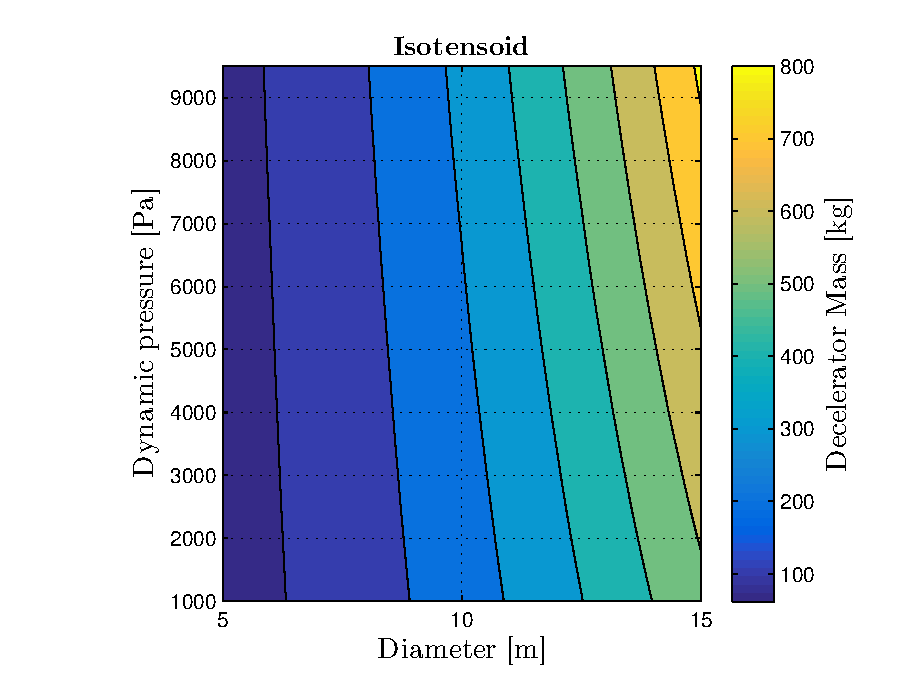
\includegraphics[width = 1.0\textwidth]{Figure/ISO_comp.eps}
\caption{\acrlong{dot} for mission duration}
\label{fig:dotduration}
\end{figure}
